%%%%%%%%%%%%%%%%%%%%%%%%%%%%%%%%%%%%%%%%%%%%%%%%%%%%%%%%%%%%%%%%%%%%%%%%%%%%%%%%%%%%
% Template for STAT 548 Qualifying Paper Report
% Author: Ben Bloem-Reddy <benbr@stat.ubc.ca>
% Revised: Daniel J. McDonald <daniel@stat.ubc.ca>
% Date: 20 August 2022
%%%%%%%%%%%%%%%%%%%%%%%%%%%%%%%%%%%%%%%%%%%%%%%%%%%%%%%%%%%%%%%%%%%%%%%%%%%%%%%%%%%%

% Note: You will get an empty bibliography warning when compiling until you include a citation.
\documentclass[10pt]{article}
\usepackage[autonum]{shortex}
% header.tex
% this is where you load pacakges, specify custom formats, etc.

\usepackage[margin=0.9in,footskip=25pt]{geometry} 
% \usepackage{changepage}
\usepackage{amsmath,amsthm,amssymb,amsfonts}
\usepackage{mathtools}
% enumitem for custom lists
\usepackage{enumitem}
% Load dsfont this to get proper indicator function (bold 1) with \mathds{1}:
\usepackage{dsfont}
\usepackage{centernot}

\usepackage[usenames,dvipsnames]{xcolor}

% set up commenting code (I will use this during marking)
\definecolor{CommentColor}{rgb}{0,.50,.50}
\newcounter{margincounter}
\newcommand{\displaycounter}{{\arabic{margincounter}}}
\newcommand{\incdisplaycounter}{{\stepcounter{margincounter}\arabic{margincounter}}}
\newcommand{\COMMENT}[1]{\textcolor{CommentColor}{$\,^{(\incdisplaycounter)}$}\marginpar{\scriptsize\textcolor{CommentColor}{ {\tiny $(\displaycounter)$} #1}}}

\usepackage{appendix}

% set up graphics
\usepackage{graphicx}
\DeclareGraphicsExtensions{.pdf,.png,.jpg}
\graphicspath{ {fig/} }


\usepackage[sort&compress,round]{natbib}

%%%%%%%%%%%%%%%%%%%%%%%%%%%%%%%%%%%%%%%%%%%%%%%%%%%%%%%%%%%%%%%%%%%%%%%%%%%%%%%%%%%%
% most other packages you might use should be loaded before hyperref
%%%%%%%%%%%%%%%%%%%%%%%%%%%%%%%%%%%%%%%%%%%%%%%%%%%%%%%%%%%%%%%%%%%%%%%%%%%%%%%%%%%%

% Set up hyperlinks:
\definecolor{RefColor}{rgb}{0,0,.65}
\usepackage[colorlinks,linkcolor=RefColor,citecolor=RefColor,urlcolor=RefColor]{hyperref}

\usepackage[capitalize]{cleveref}
\crefname{appsec}{Appendix}{Appendices} % you can tell cleveref what to call things
% defs.tex
% this is where you define custom notation, commands, etc.


%%
% full alphabets of different styles
%%

% bf series
\def\bfA{\mathbf{A}}
\def\bfB{\mathbf{B}}
\def\bfC{\mathbf{C}}
\def\bfD{\mathbf{D}}
\def\bfE{\mathbf{E}}
\def\bfF{\mathbf{F}}
\def\bfG{\mathbf{G}}
\def\bfH{\mathbf{H}}
\def\bfI{\mathbf{I}}
\def\bfJ{\mathbf{J}}
\def\bfK{\mathbf{K}}
\def\bfL{\mathbf{L}}
\def\bfM{\mathbf{M}}
\def\bfN{\mathbf{N}}
\def\bfO{\mathbf{O}}
\def\bfP{\mathbf{P}}
\def\bfQ{\mathbf{Q}}
\def\bfR{\mathbf{R}}
\def\bfS{\mathbf{S}}
\def\bfT{\mathbf{T}}
\def\bfU{\mathbf{U}}
\def\bfV{\mathbf{V}}
\def\bfW{\mathbf{W}}
\def\bfX{\mathbf{X}}
\def\bfY{\mathbf{Y}}
\def\bfZ{\mathbf{Z}}

% bb series
\def\bbA{\mathbb{A}}
\def\bbB{\mathbb{B}}
\def\bbC{\mathbb{C}}
\def\bbD{\mathbb{D}}
\def\bbE{\mathbb{E}}
\def\bbF{\mathbb{F}}
\def\bbG{\mathbb{G}}
\def\bbH{\mathbb{H}}
\def\bbI{\mathbb{I}}
\def\bbJ{\mathbb{J}}
\def\bbK{\mathbb{K}}
\def\bbL{\mathbb{L}}
\def\bbM{\mathbb{M}}
\def\bbN{\mathbb{N}}
\def\bbO{\mathbb{O}}
\def\bbP{\mathbb{P}}
\def\bbQ{\mathbb{Q}}
\def\bbR{\mathbb{R}}
\def\bbS{\mathbb{S}}
\def\bbT{\mathbb{T}}
\def\bbU{\mathbb{U}}
\def\bbV{\mathbb{V}}
\def\bbW{\mathbb{W}}
\def\bbX{\mathbb{X}}
\def\bbY{\mathbb{Y}}
\def\bbZ{\mathbb{Z}}

% cal series
\def\calA{\mathcal{A}}
\def\calB{\mathcal{B}}
\def\calC{\mathcal{C}}
\def\calD{\mathcal{D}}
\def\calE{\mathcal{E}}
\def\calF{\mathcal{F}}
\def\calG{\mathcal{G}}
\def\calH{\mathcal{H}}
\def\calI{\mathcal{I}}
\def\calJ{\mathcal{J}}
\def\calK{\mathcal{K}}
\def\calL{\mathcal{L}}
\def\calM{\mathcal{M}}
\def\calN{\mathcal{N}}
\def\calO{\mathcal{O}}
\def\calP{\mathcal{P}}
\def\calQ{\mathcal{Q}}
\def\calR{\mathcal{R}}
\def\calS{\mathcal{S}}
\def\calT{\mathcal{T}}
\def\calU{\mathcal{U}}
\def\calV{\mathcal{V}}
\def\calW{\mathcal{W}}
\def\calX{\mathcal{X}}
\def\calY{\mathcal{Y}}
\def\calZ{\mathcal{Z}}


%%%%%%%%%%%%%%%%%%%%%%%%%%%%%%%%%%%%%%%%%%%%%%%%%%%%%%%%%%
% text short-cuts
\def\iid{i.i.d.\ } %i.i.d.
\def\ie{i.e.\ }
\def\eg{e.g.\ }
\def\Polya{P\'{o}lya\ }
%%%%%%%%%%%%%%%%%%%%%%%%%%%%%%%%%%%%%%%%%%%%%%%%%%%%%%%%%%

%%%%%%%%%%%%%%%%%%%%%%%%%%%%%%%%%%%%%%%%%%%%%%%%%%%%%%%%%%
% quasi-universal probabilistic and mathematical notation
% my preferences (modulo publication conventions, and clashes like random vectors):
%   vectors: bold, lowercase
%   matrices: bold, uppercase
%   operators: blackboard (e.g., \mathbb{E}), uppercase
%   sets, spaces: calligraphic, uppercase
%   random variables: normal font, uppercase
%   deterministic quantities: normal font, lowercase
%%%%%%%%%%%%%%%%%%%%%%%%%%%%%%%%%%%%%%%%%%%%%%%%%%%%%%%%%%

% operators
\def\P{\bbP} %fundamental probability
\def\E{\bbE} %expectation

\newcommand{\Expect}[1]{\E \left{ #1\right}}
% conditional expectation
\DeclarePairedDelimiterX\bigCond[2]{[}{]}{#1 \;\delimsize\vert\; #2}
\newcommand{\conditional}[3][]{\E_{#1}\bigCond*{#2}{#3}}
\def\Law{\mathcal{L}} %law; this is by convention in the literature
\def\indicator{\mathds{1}} % indicator function

% norms
\newcommand{\norm}[1]{\left\lVert #1 \right\rVert}

% binary relations
\def\condind{{\perp\!\!\!\perp}} %independence/conditional independence
\def\equdist{\stackrel{\text{\rm\tiny d}}{=}} %equal in distribution
\def\equas{\stackrel{\text{\rm\tiny a.s.}}{=}} %euqal amost surely
\def\simiid{\sim_{\mbox{\tiny iid}}} %sampled i.i.d

% common vectors and matrices
\def\onevec{\mathbf{1}}
\def\iden{\mathbf{I}} % identity matrix
\def\supp{\text{\rm supp}}

% misc
% floor and ceiling
\DeclarePairedDelimiter{\ceilpair}{\lceil}{\rceil}
\DeclarePairedDelimiter{\floor}{\lfloor}{\rfloor}
\newcommand{\argdot}{{\,\vcenter{\hbox{\tiny$\bullet$}}\,}} %generic argument dot
%%%%%%%%%%%%%%%%%%%%%%%%%%%%%%%%%%%%%%%%%%%%%%%%%%%%%%%%%%

%%%%%%%%%%%%%%%%%%%%%%%%%%%%%%%%%%%%%%%%%%%%%%%%%%%%%%%%%%
%% some distributions
% continuous
\def\UnifDist{\text{\rm Unif}}
\def\BetaDist{\text{\rm Beta}}
\def\ExpDist{\text{\rm Exp}}
\def\GammaDist{\text{\rm Gamma}}
\def\NormalDist{\text{\rm Normal}}


% discrete
\def\BernDist{\text{\rm Bernoulli}}
\def\BinomDist{\text{\rm Binomial}}
\def\PoissonDist{\text{\rm Poisson}}
%%%%%%%%%%%%%%%%%%%%%%%%%%%%%%%%%%%%%%%%%%%%%%%%%%%%%%%%%%

%%%%%%%%%%%%%%%%%%%%%%%%%%%%%%%%%%%%%%%%%%%%%%%%%%%%%%%%%%
% Project-specific notation should go here
% (Because it's at the end of the file, it can overwrite anything that came before.)



%%%%%%%%%%%%%%%%%%%%%%%%%%%%%%%%%%%%%%%%%%%%%%%%%%%%%%%%%%



%%%%%%%%%%%%%%%%%%%%%%%%%%%%%%%%%%%%%%%%%%%%%%%%%%%%%%%%%%%%%%%%%%%%%%%%%%%%%%%%%

% your title/author/date information go here
\title{Qualifying Paper Report for Adjusting COVID-19 Seroprevalence Survey Results to Account for Test
Sensitivity and Specificity} % replace with your title, a meaningful title
\author{Naitong Chen} % replace with your name
\date{\today} % replace with your submission date


% start of document
\begin{document}

\maketitle

\section{Introduction}
Over the past few years, tracking the spread of COVID-19 has been crucial to developing a scientific understanding the disease, which ultimately guided public health protocols aimed at controlling the spread of the disease across the world. As with any epidemic/pandemic, reported case counts wthin a defined geographic region is one of the most accessible statistics indicating the scale of the spread of a disease. However, due to testing availability, there may be many individuals in a given region that have been infected but not tested. This means that the total number of infection may be much greater than that reflected from reported case counts \citep{byambasuren2021comparison}.\\
\newline$ $
To more accuratly estimate the cumulative number of infections over a period of time, an alternative approach is to conduct population-based seroprevalence studies. To carry out a seroprevalence study for a given region on a given disease, researchers begin by obtaining a sample representative of the population. Antibody tests are then performed for the disease of interest over each individual in the sample. A positive antibody test indicates a case of infection of the tested disease. Therefore, the proportion of positive tests in the sample can be used as an estimate of the porportion of population infected with the disease over some time interval, which we call the cumulative incidence. Given the population size of the corresponding region, one can estimate the total number of infected individuals in the population using the estimated cumulative incidence. It is worth noting, however, that seroprevalence studies cannot identify previous infections whose antibodies are no longer detectable or recent infections that have yet to produce detectable antibodies. At the same time, they also do not include individuals that have died after becoming infected. As a result, a seroprevalence study as we describe it here is only informative about cumulative incidence for the average period, prior to sample collection, over which antibodies are detectable, provided that the disease has a relatively low fatality rate.\\
\newline$ $
We know that COVID-19 has a relatively low fatality rate. In fact, it is estimated to be around $2.5$\% in the US by \cite{khafaie2020cross}. We also know that an individual starts to produce detectable antibodies after an average of 25 days since infection, and that the antibodies stay detectable for months after infection \citep{sethuraman2020interpreting,choe2021antibody}. Therefore, using data from a seroprevalence study conducted within the first few months of the COVID-19 pandemic, we can estimate cumulative incidence over the period from the beginning of the pandemic until roughly a month prior to when the samples were taken.
\subsection{Adjusting for test-kit performance}
Since antibody tests are not 100\% accurate, there may be positive cases that test negative and negative cases that test positive. Therefore, one would ideally also like to adjust cumulative incidence for test-kit performance. This is typically done as follows. We begin by defining test specificity $sp$ as the proportion of noncases that test negative and test sensitivity $se$ as the proportion of actual cases that test positive. Then with the true cumulative incidence being denoted as $s$, we can write the observed prevalence $p$, which describes the proportion of population that would test positive for antibodies to the virus that causes the disease of interest, as
\[
p = s \times se + (1-s) \times (1 - sp).
\]
To put in words, the observed prevalence can be decomposed into the proportion of actual cases that correctly test positive and noncases that incorrectly test positive. There are multiple approaches for incorporating this test-kit performance adjustment into the analysis of seroprevalence data. \cite{meyer2022adjusting} proposes a novel Bayesian model that adjusts cumulative incidence for test-kit performance. This method is then applied to a dataset from a COVID-19 seroprevalence study (based on detection of SARS-Cov-2 IgG) conducted in New York state in early 2020. We walk through the construction of this method in the following section.
\section{A Bayesian Approach to Analyzing Seroprevalence Data}
Given the total sample size $n$ from some region and the number of positive tests $x$ from the sample, we can follow the above test-kit performance adjustment and model the number of positive tests as the outcome of a Binomial distribution with the total sample size as the number of trials and observed prevalence as the probability of success, i.e.,
\[
x \given n, s, se, sp \distas \distBinom\left(n, s \times se + (1-s) \times (1 - sp)\right) = \distBinom(n, p).
\]
Using the above as the likelihood function of $s, se$ and $sp$, we can construct a Bayesian model by defining a set of prior distributions on each of $s, se$, and $sp$ using distributions whose support is on $[0,1]$. These prior distributions represent our apriori knowledge about these quantities. The prior and the likelihood together lead to a posterior distribution (conditional distribution given observed data) of $s$, which we can use to describe our belief on the cumulative incidence updated by observing the data at hand. 
\subsection{Deploying the Bayesian model}
\cite{meyer2022adjusting} applies this bayesian model to a dataset obtained from a seroprevalence study conducted in New York state between April 19 and April 28 in 2020. This dataset contains the number of positive antibody tests and the total number of tests from each of the 11 regions across New York state in the study. Full details of data can be found in \cite{rosenberg2020cumulative}. With consideration of the average time between infection and when antibodies become detectable, this dataset can be used to estimate cumulative incidences from the beginning of the pandemic until Mar 29, 2020. This is because there are 25 days between Mar 29, 2020 and the seroprevalence study midpoint April 23, 2020.\\
\newline$ $
Instead of directly applying the above Bayesian model where each region gets its own prior on cumulative incidence, \cite{meyer2022adjusting} remarks it is possible that regions close to each other geographically may share sociodemographic factors which are associated with the number of infections. As a result, \cite{meyer2022adjusting} groups the 11 regions into three super-regions (New York City, Westchester and Rockland Counties and Long Island, as well as rest of state), with regions from the same super-region sharing a common prior distribution on their cumulative incidences. Denoting $s_{ij}, p_{ij}, n_{ij}$ and $x_{ij}$ as the cumulative incidence, observed incidence, number of samples, and number of positive antibody tests from the $i^\text{th}$ region in the $j^\text{th}$ super-region, the final Bayesian model is defined as follows.
\[
s_{i1} &\distiid \distBeta(2.1792, 9.8208) \quad \forall i \text{ in super-region} 1 \text{ (New York City)},\\
s_{i2} &\distiid \distBeta(2.6641, 9.3359) \quad \forall i \text{ in super-region} 2 \text{ (Westchester, Rockland Counties and Long Island)},\\
s_{i3} &\distiid \distBeta(1.1930, 10.8070) \quad \forall i \text{ in super-region} 3 \text{ (rest of state)},\\
se &\distas \distBeta(205, 29)_{\{0.8, 0.95\}},\\
sp &\distas \distBeta(288, 2)_{\{0.9, 1\}},\\
p_{ij} &= s_{ij} \times se + (1-s_{ij}) \times (1 - sp), \quad \forall i, j\\
x_{ij} \given n_{ij}, p_{ij} &\distind \distBinom(n_{ij}, p_{ij}) \quad \forall i, j.
\]
The priors for each region are chosen so that the mean of the prior matches the ratio between the cumulative reported case count up until March 29, 2020 and the total population of the corresponding super-region. On the other hand, the priors on test sensitivity and test specificity are based on validation studies: \cite{rosenberg2020cumulative} estimates the test specificity to be $0.9975$ with a 95\% confidence interval of $[0.961, 1]$, and the test sensitivity to be $0.879$ with a 95\% confidence interval of $[0.837, 0.921]$. The priors are then chosen so that means and variances of the priors on test specificity and sensitivity to match the results from the validation studies. Note that the subscripts denote truncation to the specified regions.\\
\newline$ $
Suppose that there are $r_j$ regions in the $j^\text{th}$ super-region, we can write density of the target posterior distribution as
\[
p(S, se, sp \given X, N) = \frac{1}{Z}p(se)p(sp)\prod_{j=1}^3\prod_{i=1}^{r_j} p(s_{ij})p(x_{ij}\given sp, se, s_{ij}),
\]
where $p(\cdot)$ is the prior density corresponding to each parameter of interest, $p(\cdot \given \cdot)$ is the likelihood, and $Z$ is the normalization constant. Also note that $S$, $X$ and $N$ denote vectors containing the cumulative incidence, number of positive tests in the sample, and total sample size for each region considered in the study. With the model specified, we can use Markov Chain Monte Carlo to obtain samples from the posterior distribution of regional cumulative incidences as well as test specificity and sensitivity. Given a set of regional cumulative incidences from the posterior distribution, we can estimate the cumulative incidence for each super-region or the entire state using the average over the corresponding regional cumulative incidences weighted by the proportion of population living in each region. \cite{meyer2022adjusting} uses the median values over $400,000$ posterior samples as point estimates for each parameter of interest. At the same time, equal tailed 95\% credible intervals, which cover 95\% of the area under the corresponding posterior densities, are used to quantify the uncertainty about the estimates.
\subsection{Related frequentist approaches}
\cite{meyer2022adjusting} compares the results from the above Bayesian model to a non-Bayesian version of the same analysis. In the non-Bayesian version of the analysis, given a specific region (or super-region, or the entire state), with the sample proportion of positive tests being denoted $\hat{p}$, we can estimate the cumulative incidence of that region by rearranging the equation that adjusts for test specificity and sensitivity.
\[
p = s \times se + (1-s) \times (1 - sp) \implies \hat{s} = (\hat{p} + sp - 1) / (se + sp - 1).
\]
Note that here the sample proportion of positive tests plays the same role as observed prevalence in the Bayesian version of the analysis. The point estimate of the cumulative incidence is obtained by plugging in the estimated test specificity and sensitivity values from the validation studies. To quantify the uncertainty around each point estimate in terms of test-kit performance, \cite{meyer2022adjusting} constructs an iterval using the 95\% confidence interval endpoints from the validation studies. Let $\hat{se}, \hat{sp}$ denote the point estimates for test sensitivity and specificity from the validation studies, with the corresponding 95\% confidence intervals being $[se_l, se_u]$ and $[sp_l, sp_u]$. The uncertainty interval associated with $s$ can be written as
\[
[(\hat{p} + sp_l - 1) / (se_u + sp_l - 1), \quad &(\hat{p} + sp_u - 1) / (se_l + sp_u - 1)].
\] 
In particular, the lowerbound of this above interval is obtained by plugging in the lower endpoint of test specificity and upper endpoint of test sensitivity, and vice versa. It is worth noting, however, that this interval is not a 95\% confidence interval around the true cumulative incidence of the corresponding region.\\
\newline$ $
Alternatively, \cite{rosenberg2020cumulative} takes on a different approach quantifying the uncertainty around each estimated cumulative incidence. The procedure can be summarized as follows. Given the number of positive tests as well as total sample size in a region, we can construct a 95\% confidence interval on the observed prevalence for that given region. We denote this interval $[p_l, p_u]$. To incorporate the uncertainty of test-kit performance, we can construct the following three sets of 95\% confidence intervals on the cumulative incidence
\[
[(p_l + \hat{sp} - 1) / (\hat{se} + \hat{sp} - 1), \quad &(p_u + \hat{sp} - 1) / (\hat{se} + \hat{sp} - 1)],\\
[(p_l + sp_l - 1) / (se_u + sp_l - 1), \quad &(p_u + sp_l - 1) / (se_u + sp_l - 1)],\\
[(p_l + sp_u - 1) / (se_l + sp_u - 1), \quad &(p_u + sp_u - 1) / (se_l + sp_u - 1)].
\]
In the above three intervals, the first one corresponds to the average test-kit performance obtained from the validation studies, the second interval corresponds to the worst case of combined test-kit performance, and the third interval corresponds to the best case of combined test-kit performance.\\
\newline$ $
Comparing the results from both studies, we can see that the point estimates from both the Bayesian and non-Bayesian analyses are relatively similar, but the Bayesian credible intervals are generally narrower than the intervals constructed using confidence interval endpoints. In addition, while some of the intervals constructed using confidence interval endpoints contain a negative lowerbound, this does not happen to any of the credible intervals constructed. A full comparison can be found in \cite{meyer2022adjusting}. In the following section, we discuss the advantages and disadvantages of the Bayesian seroprevalence analysis.
\section{Bayesian Seroprevalence Analysis Compared to its Frequentist Counterpart}
\subsection{Significance}
One of the most prominent advantages of the fully Bayesian approach to adjusting cumulative incidence for test-kit performance is that the quantified uncertainty is more interpretable compared to its non-Bayesian counterpart. This is precisely the motivation behind the development of this Bayesian procedure by \cite{meyer2022adjusting}. In the Bayesian version of the analysis, \cite{meyer2022adjusting} expresses the uncertainty of the cumulative incidence for a given region using a 95\% equal-tailed credible interval of the corresponding marginal posterior distribution. As an example, the credible interval of the cumulative incidence in the $i^\text{th}$ region in the $j^\text{th}$ super-region $s_{ij}$ can be constructed as follows. Following the notation from the previous section, we begin by writing out the marginal posterior density for $s_{ij}$:
\[
&p(s_{ij} \given X, N)\\
&\propto \int_{se}\int_{sp} p(se)p(sp) \left(\prod_{(r,q) \neq (i,j)} \int_{s_{rq}} p(s_{rq})p(x_{rq} \given n_{rq}, sp, se, s_{rq}) \partial s_{rq}\right) p(s_{ij})p(x_{ij} \given n_{ij}, sp, se, s_{ij}) \partial se \partial sp.
\]
Note that here the normalization constant is absored by proportionality. Given $p(s_{ij} \given X, N)$, the 95\% equal-tailed credible interval for $s_{ij}$ corresponds to the range of possible $s_{ij}$ values that covers the middle 95\% of the area under $p(s_{ij} \given X, N)$. In other words, if we were to sample from this marginal posterior distribution, there is a 95\% chance that the sampled value is within the credible interval. Furthermore, since the prior distribution on $s_{ij}$ ($p(s_{ij})$ in the expression of $p(s_{ij} \given X, N)$) is Beta and has support $[0,1]$, it is guaranteed by construction that the credible interval is contained in $[0,1]$.\\
\newline$ $
On the other hand, by following the non-Bayesian approach in \cite{meyer2022adjusting}, we may obtain negative estimates or uncertainty intervals that cross zero. This can be seen from the cumulative incidence correction equation in \cref{sec:frequentist}. When the sample proportion of positive tests $\hat{p}$ is smaller than $1-\hat{sp}$, the resulting estimate of the cumulative incidence would be negative. At the same time, note that the interval reprensenting the uncertainty around the estimated cumulative incidence is obtained by plugging in endpoints of two independent confidence intervals (one on test specificity and one on test sensitivity). We know that each 95\% confidence interval is a realization of all possible intervals that overall have a 95\% chance of covering what is regarded as the underlying true value. Then the proportion of pairs of 95\% confidence intervals on test specificity and test sensitivity covering the true values simultaneously is less than 95\%. As a result, by constructing an interval through aggregating two independent 95\% confidence intervals, the resulting interval would not be a valid 95\% confidence interval. This complicates the interpretation of the resulting interval. Furthermore, uncertainty intervals constructed this way do not take into account the uncertainties around the sample proportion of positive tests. While the other approach in \cite{rosenberg2020cumulative} takes into account both the uncertainties of the sample proportion of positive tests as well as test-kit performance, the use of three intervals still makes the quantified uncertainty not as easily interpreted as that under the Bayesian framework. Finally, we note that this approach may still result in negative estimated cumulative incidences.

\subsection{Limitations and challenges}
We begin by clarifying the notion of hierarchical priors. \cite{meyer2022adjusting} claims that the model they have constructed entails a hierarchical prior structure. However, this is not the case. The simplest Bayesian hierarchical models contain three layers: likelihood of the parameter of interest given data, a prior distribution that governs the parameter of interest, and a hyper-prior distribution that governs the prior distribution. However, the Bayesian model defined in \cite{meyer2022adjusting} does not contain any hyper-prior distributions that govens the prior distribution on cumulative incidence, test specificity, or test sensitivity. Therefore, while the Bayesian model constructed in \cite{meyer2022adjusting} does leverage prior information unique to each super-region, the use of the term hierarchical prior here is not precise.\\
\newline$ $
Following up on use of prior distributions that are unique to each super-region, the grouping of regions into super-regions remain somewhat arbitrary. For example, \cite{meyer2022adjusting} does not provide an argument for combining Westchester and Rockland Counties with Long Island into one super-region. It would be of interest to know how sensitive the Bayesian model is to the grouping of regions into super-regions. After the structure of the model is determined, we still need to consider the sensitivity of the model to prior specification. While \cite{meyer2022adjusting} tested a set of non-informative, weakly informative, and informative priors on the regional cumulative incidences, the same sensitivity analysis should ideally be carried out for test sensitivity and test specificity as well. This is because there are vast variabilities among estimated COVID-19 antibody test sensitivity and specificity from different studies. As an example, test sensitivity is estimated to be as low as $28$\% in \cite{noordin2022sero}. Should there be a clear difference in the resulting estimates, further investigations need be carried out in order to produce reliable estimates of cumulative incidences for each region.\\
\newline$ $
Finally, we note that both the Bayesian and non-Bayesian analyses considered here do not account for seroreversion, which is the loss of antibody detectability. As we obtain seroprevalence data from later stages of the pandemic, we run into higher risks of underestimating the proportion of population previously infected by COVID-19. This is because antibodies for the virus that causes COVID-19 may become undetectable after some period of time since infection. Individuals who have seroreverted would not count towards the sample proportions of positive antibody tests. However, it is important to account for these individuals in many cases. An example is when the goal is to estimate the case fatality rate of COVID-19, where it is crucial to include those who have seroreverted to avoid overestimating the case fatality rate \citep{brazeau2022estimating}. As a result, both the Bayesian and non-Bayesian analyses discussed above do not generalize to seroprevalence studies conducted later on in the pandemic as one might have hoped. In the following section, we propose a modification to the framework discussed above to account for seroreversion, and apply this modified Bayesian model to a serial seroprevalence study conducted in Quebec, Canada between 2020 and 2021.
\section{Bayesian Seroprevalence Analysis with Seroreversion Correction}
In a serial seroprevalence study conducted in Quebec, Canada by \cite{lewin2021sars} and \cite{lewin2022seroprevalence}, a procedure for seroreversion correction is applied in a non-Bayesian analysis. Here we begin by describing the dataset used in this analysis before illustrating the procedure used to adjust estimated cumulative incidences for seroreversion.
\subsection{Data}
The datasets used in \cite{lewin2021sars} and \cite{lewin2022seroprevalence} together can be viewed as one for a serial COVID-19 seroprevalence study in Quebec, Canada. For both phases of the study, numbers of antibody-positive samples as well as total number of samples are recorded for each of the three regions in Quebec: Montreal-Laval region, region surrounding Montreal-Laval, as well as other regions. Phase I of the study was conducted relatively early in the pandemic, and it collected samples obtained between May 25 and July 9, 2020. Phase II of the study contains samples collected from  January 25 to Mar 11, 2021.\\
\newline $ $
While we can use the data from phase I of the study to estimate regional cumulative incidences in Quebec between the beginning of the pandemic until around May 23, 2020 (accounting for the average 25 days between infection and when antibodies become detectable), simply repeating the same analysis using data from phase II of the study likely would not result in valid estimates of cumulative incidences between the beginning of the pandemic and the beginning of 2021. This is because there had already been almost a year since the beginning of the pandemic by the time when phase II samples were collected. Some of the individuals may have had a previous infection but had seroreverted by the time of sample collection. Consequently, the raw estimates may be lower than the true cumulative incidence of a given region. As a result, to account for seroreversion when analyzing data from phase II of the seroprevalence study, \cite{lewin2022seroprevalence} also conducted a seroreversion substudy. In particular, a number of the individuals who tested postive for SARS-Cov-2 antibodies during phase I of the study were tested again in 2021. The number of these individuals as well as the number of positive tests were recorded. The data from both phases of the study are summarized in \cref{tab:dat}.\\
\newline $ $
It is important to point out that the phase II data presented here only concern the unvaccinated population. While data for both those who were and were not vaccinated are presented in \cite{lewin2022seroprevalence}, we have chosen to focus on the unvaccinated population since none of the vaccinated individuals had seroreverted at the time and so it is not necessary for adjust for seroreversion. Finally, we note that for the remainder of the report, any notation that is redefined from the previous sections are within the context of the seroprevalence study in Quebec.

\begin{table}[]
\centering
\begin{tabular}{c|cc|cc|cc}
                           & \multicolumn{2}{c}{\textbf{Phase I}} & \multicolumn{2}{c}{\textbf{Phase II (unvaccinated)}} & \multicolumn{2}{c}{\textbf{Seroreversion substudy}}\\
                           & reactive      & tested      & reactive              & tested      & seroreverted              & tested        \\
                           \hline
Montreal-Laval             & 90            & 3061        & 48                    & 1925      & - & -          \\
Surrounding Montreal-Laval & 48            & 1925        & 128                   & 1422   & - & -             \\
Other                      & 35            & 2705        & 372                   & 4304          & - & -      \\
\hline
Total                      & 173           & 7691        & 715                   & 7304          &    32 & 109  
\end{tabular}
\caption{Seroprevalence data from \cite{lewin2021sars} and \cite{lewin2022seroprevalence}. Reactive indicates the number of positive tests against SARS-Cov-2 IgG.}
\label{tab:dat}
\end{table}
\subsection{Adjusting for seroreversion}
As mentioned above, not correcting for seroreversion when conducting seroprevalence analysis on data from phase II of the above mentioned study may result in unreliable estimates of regional cumulative incidences. This is because such analyses fail to account for those who have had a previous infection but had already seroreverted by the time of sample collection. Luckily, with the data from phase I of the study, for each region in Quebec, we can produce a valid estimate of the cumulative incidence between the beginning of the pandemic and May 2020. Additionally, from the seroreversion substudy, we can estimate the proportion of the antibody-positive population from phase I of the study that had seroreverted by phase II of the study. As a result, \cite{lewin2022seroprevalence} adjusts the raw estimate of cumulative incidence from phase II by adding the product of the estimated cumulative incidence from phase I and the estimated proportion that have seroreverted. Mathematically, let $\hat{s}_{prev}$ be the estimated cumulative incidence of a region in Quebec from phase I, $\hat{p}$ be the estimated observed prevalence (proportion of positive samples) from phase II, and $\hat{sr}$ be the observed proportion of seroreversion, we can estimate the cumulative incidence between the beginning of the pandemic and the beginning of 2021 using
\[
\hat{s} = \hat{p} + \hat{s}_{prev} \times \hat{sr}.
\]
To quantify the uncertainty around $\hat{s}$, we begin by noting that there are three sources of uncertainty: the estimated cumulative incidence from phase I, the observed prevalence from phase II, and the proportion of seroreversion. Note that here the cumulative incidence from phase I is directly estimated using the observed prevalence from phase I. For some arbitrary proportion of interest $t$ estimated by $\hat{t} = \frac{x}{n}$, where $x$ and $n$ denote the number of positive samples and the total sample size, we can construct a $95$\% confidence interval by
\[
\left[ \hat{t} - Q(0.975) \times \sqrt{\frac{\hat{t}(1-\hat{t})}{n}}, \quad \hat{t} + Q(0.975) \times \sqrt{\frac{\hat{t}(1-\hat{t})}{n}} \right],
\]
where $Q$ is the quantile function of the standard normal distribution. Following this procedure, we can construct individual 95\% confidence intervals for the cumulative incidence from phase I $s_{prev}$ and observed prevalence from phase II $p$, as well as the proportion of seroreversion $sr$. Write these intervals as
\[
[s_{prev, l},\quad s_{prev, u}], \quad [p_{l},\quad p_{u}], \quad [sr_{l},\quad sr_{u}].
\]
Then to construct an uncertainty interval for $s$, we can aggregate the above three 95\% confidence intervals using combinations of the confidence interval endpoints that give the lowest and highest estimated cumulative incidence
\[
[p_l + s_{prev, l} \times sr_{l}, \quad p_u + s_{prev, u} \times sr_{u}].
\]
Again, the above interval is not a valid $95$\% confidence interval, but it nonetheless quantifies the scale of uncertainty.\\
\newline$ $
We can easily extend the model above and incorporate adjustment for test-kit performance. This is achieved by writing, with $p_{prev}$ denoting the observed prevalence in phase I,
\[
p_{prev} = s_{prev} \times se + (1-s_{prev}) \times (1 - sp) &\implies s_{prev} = \frac{p_{prev} + sp - 1}{se + sp - 1},\\
p = (s - sr \times s_{prev}) \times se + (1 - (s - sr \times s_{prev})) \times (1 - sp) &\implies s = \frac{p+1-sp}{se+sp-1} + sr \times s_{prev}.
\]
In this above formulation of observed prevalence from phase II ($p$), we first substract from the true cumulative incidence the proportion that have seroreverted from the true seroprevalence, and then adjust for test-kit performance. This is because the test-kit only has a chance at detecting antibodies if the subject has not yet seroreverted. Using the same approach to aggregate over all sources of uncertainty, we arrive at the estimated cumulative incidence for a given region between the beginning of the pandemic and the beginning of 2021
\[
\hat{s} = \frac{\hat{p}+1-\hat{sp}}{\hat{se}+\hat{sp}-1} + \hat{sr} \times \hat{s}_{prev}
\]
with a corresponding uncertainty interval adjusting for both seroreversion and test-kit performance
\[
\left[\frac{p_l+1-sp_l}{se_u+sp_l-1} + sr_l \times s_{prev,l}, \quad \frac{p_u+1-sp_u}{se_l+sp_u-1} + sr_u \times s_{prev, u} \right],\\
\]
Note that
\[
s_{prev,l} = (p_{prev,l} + sp_l - 1) / (se_u - 1 + sp_l), \quad s_{prev,u} = (p_{prev,u} + sp_u - 1) / (se_l - 1 + sp_u).
\]
Finally, we note that if we had data on the unvaccinated population from each of the three regions in Quebec, we could obtain a province-wide estimate of the cumulative incidence by averaging the regional cumulative incidences weighted by the proportion of population in each region. However, this information is not included in \cite{lewin2022seroprevalence}, and so our analysis here remains regional.

\subsection{Model formulation}
To maintian nice properties of Bayesian model while still accounting for seroreversion, can combine.

We can apply the approach in \cite{meyer2022adjusting} to the two datasets in \cite{lewin2021sars} and \cite{lewin2022seroprevalence} in one coherent Bayesian model that accounts for seroreversion. \\
\newline $ $
Let $s_{ij}$ denote the true seroprevalence in study $i$ and region $j$ ($i=1$ and $i=2$ correspond to first and second study, $j=1,j=2$ and $j=3$ correspond to Montreal-Laval, surrounding Montreal-Laval, and other regions). Let $P_{ij}$ denote the observed seroprevalances. Let $se, sp, sr$ denote sensitivity of test-kit, specificity of test-kit, as well as proportion of samples that has seroreverted (testing antibody-negative in 2021 but antibody-positive in 2020). Let $x_{ij}$ denote the total number of antibody-positive samples in region $j$ at study $i$, and $n_{ij}$ denote the total number of samples in region $j$ at study $i$. Finally, let $x_r$ and $n_r$ denote the total number of samples that seroreverted and the total number of samples in the seroreversion substudy. \\
\newline $ $
The model can then be written as
\[
s_{1j} &\sim \distBeta(1,1) \quad \forall j \in \{1,2,3\}\\
s_{2j} &\sim \distBeta(1, 1)_{\{ sr \times s_{1j} , 1 \}} \quad \forall j \in \{1,2,3\}\\
se &\sim \distBeta(205, 29)\\
sp &\sim \distBeta(288, 2)\\
sr &\sim \distBeta(32, 77)\\
p_{1j} &= s_{1j} \times se + (1 - s_{1j}) \times (1 - sp) \quad \forall j \in \{1,2,3\}\\
p_{2j} &= (s_{2j} - sr \times s_{1j}) \times se + (1 - (s_{2j} - sr \times s_{1j})) \times (1 - sp) \quad \forall j \in \{1,2,3\}\\
x_{ij} \given n_{ij}, p_{ij} &\distind \distBinom(n_{ij}, p_{ij}), \quad \forall i \in\{1,2\}, \quad j \in \{1,2,3\}.
\]
Following the notation from the previous section, the density of the target posterior distribution is given by
\[
p(S, se, sp, sr \given X, N) = \frac{1}{Z}p(se)p(sp)p(sr)\prod_{i=1}^3\prod_{j=1}^2 p(s_{ij})p(x_{ij}\given sp, se, sr, s_{ij}).
\]
Note that for observed seroprevalences in the first study, we adjust for test sensivitity and test specificity (Following the setup in \cite{meyer2022adjusting}. We'll likely use the same prior on $se$ and $sp$ here). For observed seroprevalences in the second study, we adjust for both test sensivitity and test specificity as well as seroreversion. Namely, we also include the proportion that have seroreverted since the first study using information from the seroreversion substudy. To ensure we do not run into negative seroprevalence estimates, we truncate $s_{21}, s_{22}, s_{23}$ accordingly.\\
\newline $ $
Altogether, this can give us an estimate of the seroprevalance in Quebec, Canada in January to March 2021 adjusting for test-kit performance as well as seroreversion.\\
\newline $ $
We can compare the results from this above Bayesian model to those from \cite{lewin2022seroprevalence} (which is not Bayesian and does not account for test-kit performance) as well a frequentist equivalence of the above Bayesian model using the same data. We can use these results to check if the claims from \cite{lewin2022seroprevalence} still hold under this different dataset, as well as to explore potential reasons as to why they do or do not hold.\\
\newline $ $
It turns out that the intervals constructed from \cite{rosenberg2020cumulative} (the non-Bayesian analysis that \cite{meyer2022adjusting} compared to) is just by using the $95\%$ confidence interval endpoints for test sensitivity and specificity to correct for the true seroprevalence using $p = s \times se + (1-s) \times (1-sp)$.

\begin{table}[]
\centering
\label{tab:results}
\begin{tabular}{c|ccc}
                           & \multicolumn{3}{c}{\textbf{Raw result}}                                        \\
                           & mean                & lowerbound             & upperbound             \\
Montreal-Laval             & 0.136               & 0.120                  & 0.154                  \\
Surrounding Montreal-Laval & 0.090               & 0.076                  & 0.106                  \\
Other                      & 0.086               & 0.078                  & 0.095                  \\
\hline
                           & \multicolumn{3}{c}{\textbf{Adjusted for seroreversion}}                          \\
                           & mean                & lowerbound             & upperbound             \\
Montreal-Laval             & 0.145               & 0.125                  & 0.168                  \\
Surrounding Montreal-Laval & 0.097               & 0.080                  & 0.119                  \\
Other                      & 0.090               & 0.080                  & 0.102                  \\
\hline
                           & \multicolumn{3}{c}{\textbf{Adjusted for seroreversion and test-kit performance}} \\
                           & mean                & lowerbound             & upperbound             \\
Montreal-Laval             & 0.161               & 0.088                  & 0.201                  \\
Surrounding Montreal-Laval & 0.107               & 0.037                  & 0.142                  \\
Other                      & 0.100               & 0.037             & 0.122                  \\
\hline
                           & \multicolumn{3}{c}{\textbf{Bayesian analysis adjusted for seroreversion and test-kit performance}}                                 \\
                           & median              & lowerbound             & upperbound             \\
Montreal-Laval             & 0.159               & 0.137                  & 0.183                  \\
Surrounding Montreal-Laval & 0.105               & 0.085                  & 0.125                  \\
Other                      & 0.096               & 0.082                  & 0.110                 
\end{tabular}
\caption{Summary of regional cumulative incidence point estimates and uncertainty intervals for all methods discussed. The first three non-Bayesian analyses contain the mean estimate as well as an uncertainty interval constructed from multiple $95$\% confidence intervals, and the last Bayesian analysis contain the median and equal-tailed $95$\% credible interval of the corresponding posterior distribution.}
\end{table}

\captionsetup[subfigure]{labelformat=empty}
\begin{figure}[ht!]
\centering
\begin{subfigure}[b]{\columnwidth} 
    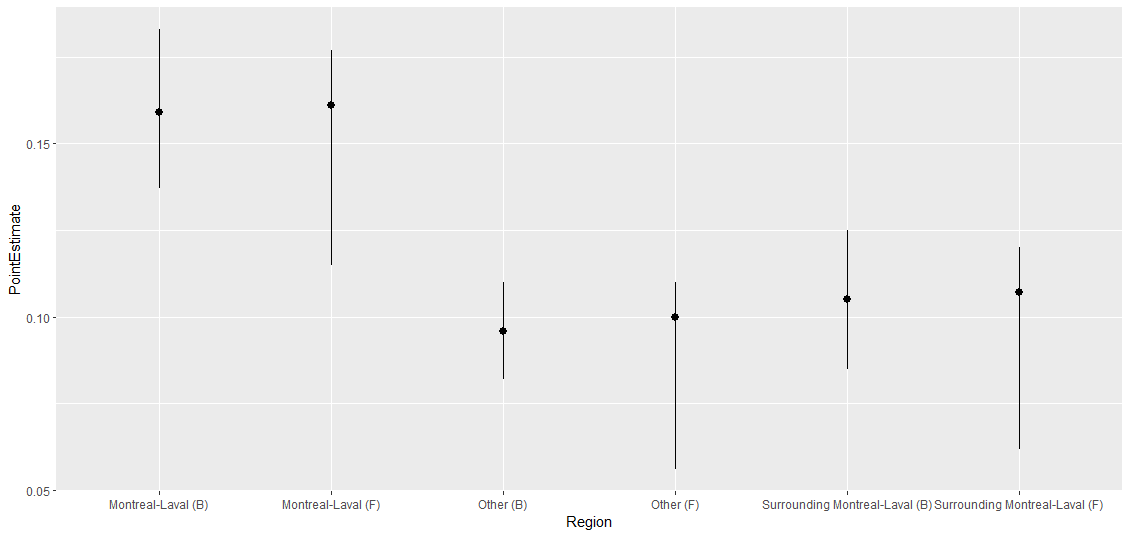
\includegraphics[width=\columnwidth]{../../plot/intervals.png}
    \caption{Comparison between uncertainty intervals for regional cumulative incidences between the Bayesian (B) and non-Bayesian (F) seroprevalence analyses, where both seroreversion and test-kit performance are accounted for.}
    \label{fig:intervals}
\end{subfigure}
\end{figure}

\subsection{Discussion of analysis results}
\section{Conclusion and Future Directions}
\cite{meyer2022adjusting} proposes a Bayesian model for conducting seroprevalence analysis that accounts for test-kit performance. By applying this model to a dataset from a seroprevalence study conducted in New York state in early 2020 and comparing the results to the non-Bayesian version of the same analysis, we see that both analyses provide similar point estimates of regional cumulative incidences. However, the Bayesian credible intervals used to quantify uncertainties around each estimate, compared to their non-Bayesian counterparts, are narrower, more interpretable, and stay well-defined (non-negative).\\
\newline$ $
In this report, we extend the above Bayesian model by incorporating the approach in \cite{lewin2022seroprevalence} to additionally account for seroreversion. By comparing the newly proposed model to its non-Bayesian counterpart using seroprevalence data from Quebec, Canada, we see that the claims in \cite{meyer2022adjusting} largely hold. Namely, the point estimates from both models are similar, with the Bayesian credible intervals being narrower and more centred around the point estimates. In fact, we do come across instances of the non-Bayesian uncertainty intervals having a lowerbound below zero.\\
\newline$ $
One of the major motivations for approaching seroprevalence analysis in a Bayesian way is to improve the interpretability of the uncertainty intervals associated with each estimated cumulative incidence. In particular, with the way that uncertainty intervals are constructed in \cite{meyer2022adjusting}, they are not valid confidence intervals. Therefore, as a future direction of research, it is of interest to develop more theoretically justified ways to aggregate individual confidence intervals to produce uncertainty intervals that remain as valid confidence intervals. One idea is to use the Bonferroni correction to adjust the confidence level of each individual confidence interval so that the resulting interval has a desired confidence level. The degree Bonferroni correction here depends on the number of individual confidence intervals (or sources of uncertainty) that we use to produce the final interval. This is based on the observation that all cumulative incidence estimators discussed in this report are strictly monotone in each parameter of interest. However, this approach does not rule out the possibility of obtaining negative point estimates or negative uncertainty interval endpoints.\\
\newline$ $
Another direction for future research involves more formally testing the sensitivity of the proposed Bayesian models to the specification of prior distributions. As discussed before, the prior on cumulative incidences are based on cumulative reported case counts, and test sensitivity, test specificity, as well as seroreversion proportion are based on (external) validation studies. These sources of prior distributions contain variabilities within themselves, and so it is crucial to assess prior sensitivity beyond merely testing a number of plausible prior specifications. Should the model be sensitive to prior specification, more investigation may be conducted to help stablize the output of the corresponding Bayesian models.


\bibliographystyle{plainnat}
\bibliography{../references/qp.bib}

\appendix
\section{Supplementary Material}

\end{document}
